\documentclass[11pt,a4j]{jsarticle}
\usepackage{float,array,booktabs,here}
\usepackage{amsmath}
\usepackage{bm}
\usepackage[dvipdfmx]{graphicx}
% \usepackage[whole]{bxcjkjatype}%日本語もコンパイル可にする.
%\usepackage[dvipdfmx,hiresbb]{graphicx}
\usepackage[top=25truemm,bottom=25truemm,left=25truemm,right=25truemm]{geometry}

\title{Computer Vision}
\author{81819433 開放環境科学専攻情報工学専修 修士1年 飯塚 健介}
\date{\today}
\begin{document}
    \maketitle

    \section{section name}
    \subsection{subsection name}

    \section{目的と課題設定}
    私は主にセグメンテーションについて理解を深めるために授業で習った手法を用いてセグメンテーションの処理を自分で実装して
    OpenCVに備わっているライブラリ関数での実装と比較検討、また自分の実装について考察を行った。
    今回私がセグメンテーションを選んだ理由は授業中に聞いた手法でなぜセグメンテーションができるのかが気になったからである。
    また研究として深層学習のアクセラレータの開発を行うために深層学習について調べていたときに
    セグメンテーションは自動運転や医療画像の解析などにも利用されることを知ったので応用技術としても今後ますます注目されるのだろうと考えた。



    \section{開発及び実行環境}
    開発及び実行環境は次のとおりである。OpenCVは比較と入出力を受け取るために利用した。
    \begin{itemize}
        \item OS : Ubuntu18.04 
        \item 使用言語 : Python3.6.5, C++11 
        \item 使用ライブラリ : Numpy, Matplotlib, OpenCV 
       \end{itemize}

    \section{k-means法を用いたセグメンテーション}
    まず、k-means法を用いたセグメンテーションについて検討と実装を行った。

    \subsection{k-means法について}
    \cite{k-means}を参考にアルゴリズムについて検討した。k-meansではいくつのクラスタに分類するかを人が指定しなければいけない。
    そしてランダムにクラスタリングされた3次元のベクトル(画像のRGBをベクトルの各要素とした)について各クラスタの重心を求める。
    その重心から各ベクトルのユークリッド距離を算出し最小となるクラスタに属するようにする。
    これをクラスタリング結果が前回のクラスタリング結果と一致するまで、もしくはある上限回数行い、各クラスタの重心を決定する。
    ここに新たな入力ベクトルが入ってきた場合には各クラスタの重心とのユークリッド距離を算出し最小となったクラスタに属するようにする。
    具体例として、図\ref{fig:ex-kmeans-init}に示すようにランダムに生成した2次元ベクトルを基にしてクラスタの重心を求めて、
    入力データがどのクラスタに属しているかを図\ref{fig:ex-kmeans}に示す。
    バツマークがランダムに生成したベクトル、丸マークで示しているのが入力データである。
    ユークリッド距離が一番近いクラスタに分類されているのがわかる。

    \begin{figure}[H]
        \centering
        \includegraphics[clip,width=4.0cm]{img/ex-kmeans-init.jpg}
        \caption{ランダムに初期化されたベクトル\label{fig:ex-kmeans-init}}
    \end{figure} 

    \begin{figure}[H]
        \centering
        \includegraphics[clip,width=4.0cm]{img/ex-kmeans.jpg}
        \caption{k-meansによる2次元ベクトルのクラスタリングの様子\label{fig:ex-kmeans}}
    \end{figure} 

    \subsection{実装方法}
    \subsection{結果と考察}

    \section{混合ガウシアンモデルを用いたセグメンテーション}
    \subsection{混合ガウシアンモデルについて}
    混合ガウシアンモデルとは確率分布としてよく用いられる\ref{eq:gaussian}
    で示される確率分布関数を複数重ね合わせたものである。
    式で表すと\ref{eq:mixture-gaussian}である。

    具体例として、図\ref{fig:ex-mg}にランダムに生成した2次元ベクトルを基にしてクラスタの重心を求めて、
    入力データがどのクラスタに属しているかを図\ref{fig:ex-kmeans}に示す。
    バツマークがランダムに生成したベクトル、丸マークで示しているのが入力データである。
    ユークリッド距離が一番近いクラスタに分類されているのがわかる。

    \begin{figure}[H]
        \centering
        \includegraphics[clip,width=4.0cm]{img/ex-kmeans-init.jpg}
        \caption{ランダムに初期化されたベクトル\label{fig:ex-kmeans-init}}
    \end{figure} 

    \begin{figure}[H]
        \centering
        \includegraphics[clip,width=4.0cm]{img/ex-kmeans.jpg}
        \caption{k-meansによる2次元ベクトルのクラスタリングの様子\label{fig:ex-kmeans}}
    \end{figure} 
    \subsection{実装方法}
    \subsection{結果と考察}

    \section{mean-shiftを用いたセグメンテーション}
    \subsection{mean-shiftについて}
    \subsection{実装方法}
    \subsection{結果と考察}

    \section{結論とまとめ}

    \begin{thebibliography}{9}
        \bibitem{k-means} http://home.deib.polimi.it/matteucc/Clustering/tutorial_html/kmeans.html
        \bibitem{susan} S. M. Smith and J. M. Brady,
          ``SUSAN|A new approach to low level image processing,'' Int. J. Comput.
          Vis., vol.23, no.1, pp.45-78, May 1997.
      \end{thebibliography}

    \begin{figure}[H]
      \centering
      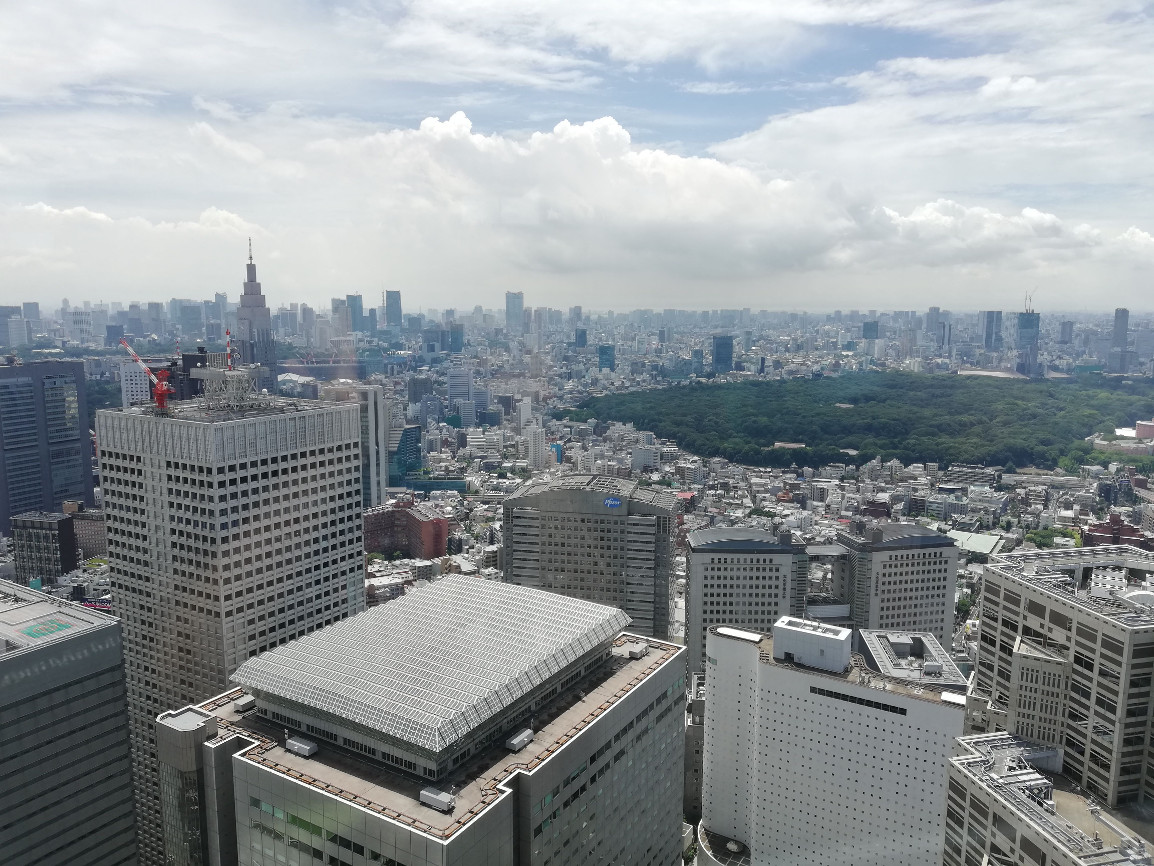
\includegraphics[clip,width=4.0cm]{img/metro.jpg}
      \caption{都庁南展望台からの写真\label{fig:cute}}
    \end{figure}

    \begin{equation}
        s\left(
        \begin{array}{c}
            u \\
            v \\
            1
        \end{array}
        \right) =
        \left(
    \begin{array}{cccc}
      P_{11} & P_{12} & P_{13} & P_{14}\\
      P_{21} & P_{22} & P_{23} & P_{24} \\
      P_{31} & P_{32} & P_{33} & P_{34} \\
    \end{array}
        \right)
        \left(
        \begin{array}{c}
            X \\
            Y \\
            Z \\
            1
        \end{array}
        \right)
        \label{eq:projection_matrix}
    \end{equation}

\end{document}
